\begin{frame}{Distancia Euclidiana en $\mathbb{R}^3$}

    \begin{columns}[c]

        %========================================
        % COLUMNA IZQUIERDA
        %========================================
        \column{0.50\textwidth}

        \begin{block}{Distancia Euclidiana}

            \centering
            \small

            \[
            R_i =
            \sqrt{
            (x_i-x)^2 +
            (y_i-y)^2 +
            (z_i-z)^2
            }
            \]

        \end{block}

        \vspace{0.25cm}

        \small
        \begin{itemize}

            \item $(x_i,y_i,z_i)$ : coordenadas conocidas del sensor $i$.

            \vspace{0.2cm}

            \item $(x,y,z)$ : posición estimada de la fuente sísmica.

            \vspace{0.2cm}

            \item $R_i$ : distancia tridimensional entre la fuente y el sensor.

        \end{itemize}

        \vspace{0.2cm}

        \begin{center}
            \small
            \textbf{
            Esta expresión mide la separación espacial entre dos puntos en $\mathbb{R}^3$.
            }
        \end{center}

        %========================================
        % COLUMNA DERECHA
        %========================================
        \column{0.46\textwidth}

        \begin{center}
            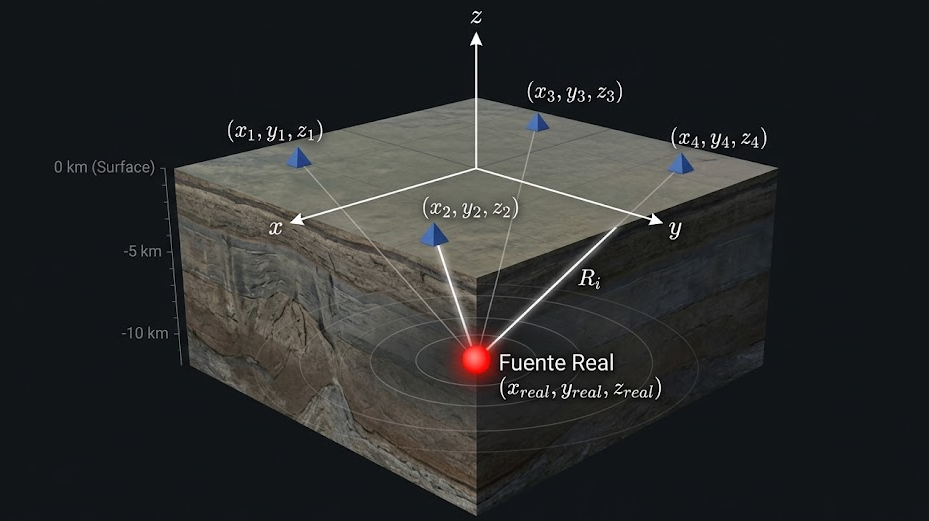
\includegraphics[width=\textwidth]{Imagenes/AtenuacioSismica.png}
        \end{center}

        \vspace{0.15cm}

        \begin{center}
            \tiny
            \textcolor{gray}{
            La geometría tridimensional permite determinar la distancia entre la fuente y cada sensor.
            }
        \end{center}

    \end{columns}

\end{frame}